%%%%%%%%%%%%%%%%%%%%%%%%%%%%%%%%%%%%%%%%%%%%%%%%%%%%%%%%%%%%%%%%%%%%%%
%%	Name: "Signal analysis template"
%%	File name: signalanalysis_template_main
%%	Version: 1.5
%%
%%	Compiler: XeLaTeX
%%
%%%%%%%%%%%%%%%%%%%%%%%%%%%%%%%%%%%%%%%%%%%%%%%%%%%%%%%%%%%%%%%%%%%%%%

\documentclass[conference,compsoc,onecolumn]{IEEEtran}

% *** LANGUAGE UTILITY PACKAGES ***
\usepackage[utf8]{inputenc} % Required for including letters with accents
\usepackage[spanish]{babel}
\usepackage{subfigure}
\usepackage{graphicx}
\usepackage{amssymb}
\usepackage{amsmath}


% *** USED PACKAGES ***
% *** MISC UTILITY PACKAGES ***
\usepackage{comment}			% Agregar comentarios
\usepackage{lipsum}				% Inserts dummy text
\usepackage{blindtext}
\usepackage{listings}					% Coding
\usepackage{verbatim}				% Verbatim
\usepackage[final]{pdfpages}
\usepackage{booktabs,dcolumn}
\usepackage{pdflscape}
\usepackage{afterpage}
%\setlist[itemize]{noitemsep, nolistsep}
\usepackage[bookmarks=false]{hyperref}
\usepackage{tcolorbox}									% Coloured boxes, for LATEX examples and theorems, etc
\usepackage{color}
\usepackage{xcolor} % Required for specifying colors by name									% Color packages foreground and back­ground color man­age­men
% *** CITATION PACKAGES ***
\usepackage{cite}
% *** GRAPHICS RELATED PACKAGES ***
\usepackage{graphicx}
\usepackage{caption}
\usepackage{pgfplots}
\usepackage{tikz}
\usetikzlibrary{shapes,arrows}
\usetikzlibrary{decorations.pathmorphing} % noisy shapes
\usetikzlibrary{fit}					% fitting shapes to coordinates
\usetikzlibrary{backgrounds}	% drawing the background after the foreground
\pgfplotsset{compat=1.13}
% *** MATH PACKAGES ***
\usepackage{amsmath}
\usepackage{mathtools}
\usepackage{amssymb}
\usepackage{amsfonts}
\usepackage{expl3}
\usepackage{bm}

% *** SPECIALIZED LIST PACKAGES ***
\usepackage{algorithmic}
\usepackage{listings}					% Coding
\usepackage[framed,numbered,autolinebreaks,useliterate]{mcode}
% *** ALIGNMENT PACKAGES ***
\usepackage{array}
% *** SUBFIGURE PACKAGES ***
%\ifCLASSOPTIONcompsoc
%\usepackage[caption=false,font=normalsize,labelfont=sf,textfont=sf]{subfig}
%\else
%\usepackage[caption=false,font=footnotesize]{subfig}
%\fi
% *** FLOAT PACKAGES ***
\usepackage{fixltx2e}
\usepackage{stfloats}
%\fnbelowfloat
%\usepackage{dblfloatfix}
% *** PDF, URL AND HYPERLINK PACKAGES ***
\usepackage{url}
\usepackage{everypage}


\usepackage{multirow} % In order to be able to insert rows spanning multiple lines
\usepackage{verbatim}
\usepackage[all]{xy}
\usepackage{listings}
\usepackage{subfigure}
\usepackage{multibib}
\usepackage{setspace} 
\usepackage{algorithm}			    	  % To insert nice algorithms

% *** CARPETA DONDE SE GUARDARAN LAS IMAGENES ***
\graphicspath{{figures/}}

% *** NUEVOS COMANDOS Y CONFIGURACIONES VARIAS ***
\interdisplaylinepenalty=2500
\newcommand{\Lpagenumber}{\ifdim\textwidth=\linewidth\else\bgroup
	\dimendef\margin=0
	\ifodd\value{page}\margin=\oddsidemargin
	\else\margin=\evensidemargin
	\fi
	\raisebox{\dimexpr -\topmargin-\headheight-\headsep-0.5\linewidth}[0pt][0pt]{%
		\rlap{\hspace{\dimexpr \margin+\textheight+\footskip}%
			\llap{\rotatebox{90}{\thepage}}}}%
	\egroup\fi}

\AddEverypageHook{\Lpagenumber}%

\newcommand{\newtxt}[1]{\textcolor{black}{#1}}
\renewcommand\IEEEkeywordsname{Palabras cláve:}
\newcommand{\mx}[1]{\mathbf{\bm{#1}}} % Matrix command
\newcommand{\vc}[1]{\mathbf{\bm{#1}}} % Vector command

%% Separación de palabras
\hyphenation{op-tical net-works semi-conduc-tor HHMMSS}

\makeatletter
\newcommand{\linebreakand}{%
  \end{@IEEEauthorhalign}
  \hfill\mbox{}\par
  \mbox{}\hfill\begin{@IEEEauthorhalign}
}
\makeatother

\begin{document}

% *** TITLES AND NAMES ***
% title of the document
\title{Reproductor de silencio}
% author names and affiliations

\author{\IEEEauthorblockN{\textsuperscript{} Andres Cubides}
\IEEEauthorblockA{\textit{Escuela de Ciencias Exactas e Ingenieria} \\
\textit{Universidad Sergio Arboleda-Bogotá, Colombia}\\
andres.cubides01@correo.usa.edu.co}
\and
\IEEEauthorblockN{\textsuperscript{} Sebastian Merchán}
\IEEEauthorblockA{\textit{Escuela de Ciencias Exactas e Ingenieria} \\
\textit{Universidad Sergio Arboleda-Bogota, Colombia}\\
sebastian.merchan01@correo.usa.edu.co}

\IEEEauthorblockN{\textsuperscript{}}
\IEEEauthorblockA{\textit{} \\
\textit{}\\}}
\maketitle

% *** MAKE TITLE ***

\IEEEoverridecommandlockouts
\IEEEpeerreviewmaketitle

\section{Idea inicial:}
Después de realizar una lluvia de ideas, la idea que más resalta su importancia sobre las demás, fue un sistema de cancelación de ruido, para diferentes entornos y ambientes, tales como:

\begin{itemize}
    \item Salas de Reunión.
    \item Hospitales.
    \item Casas.
    \item Oficinas.
    \item Universidades.
\end{itemize}

\section{Aplicación de técnicas de creatividad:}
Para tener una mayor claridad de la idea se utilizó la herramienta \textbf{SCAMPER}, donde se realizaron una serie de preguntas con el objetivo de despertar la creatividad y la innovación en la idea ya planteada. El acrónimo se resolvió de la siguiente forma.

\begin{itemize}
    \item \textbf{S - (SUSTITUIR): } Se propone sustituir las puertas, paredes y ventanas, que usualmente se utilizan para aislar el ruido externo, por un sistema electrónico de control de ruido.\\
    \item \textbf{C - (COMBINAR): } Se desea combinar dos sistemas como lo son, el sistema usual de sonido en el cual se puede elegir y reproducir musica desde una aplicación móvil, y en los momentos que no se este utilizando este sistema, cancele el ruido externo.\\
    \item \textbf{A - (ADAPTAR): } Se busca adaptar ideas como persianas o biombos, con el fin de seleccionar el espacio en el cual se desea una disminución del ruido.\\
    \item \textbf{M - (MODIFICAR): } Se modifica el uso de cancelación de ruido usual en los audífonos y headset, por un sistema para un uso colectivo.\\
    
    \item \textbf{P - (Put Other Uses - Poner otros usos): } Se ve que los bafles inteligentes y otros dispositivos de reproducción de sonido también pueden reproducir ondas invertidas anteriormente procesadas.\\

    \item \textbf{E - (Eliminar o Modificar): } El ruido o sonidos no deseados se pueden eliminar, se pueden modificar los bafles para que además de generar sonido también ayuden a silenciar el ambiente.\\
    
    \item \textbf{R - (Reordenar o Invertir): } Se puede personalizar tanto el estuche como carcasa de los micrófonos como audífonos, también los estilos y fondos de la aplicación .\\
    
    
\end{itemize}


\section{Testeo de prototipo:}
Una vez ya definida la idea es momento de probarla con los usuarios por medio de un prototipo inicial, donde se va a probar la idea, para esto se pasa a construir la idea con cartón paja y cartón, como se ve en la siguiente imagen.

\begin{figure}[H]
    \centering
    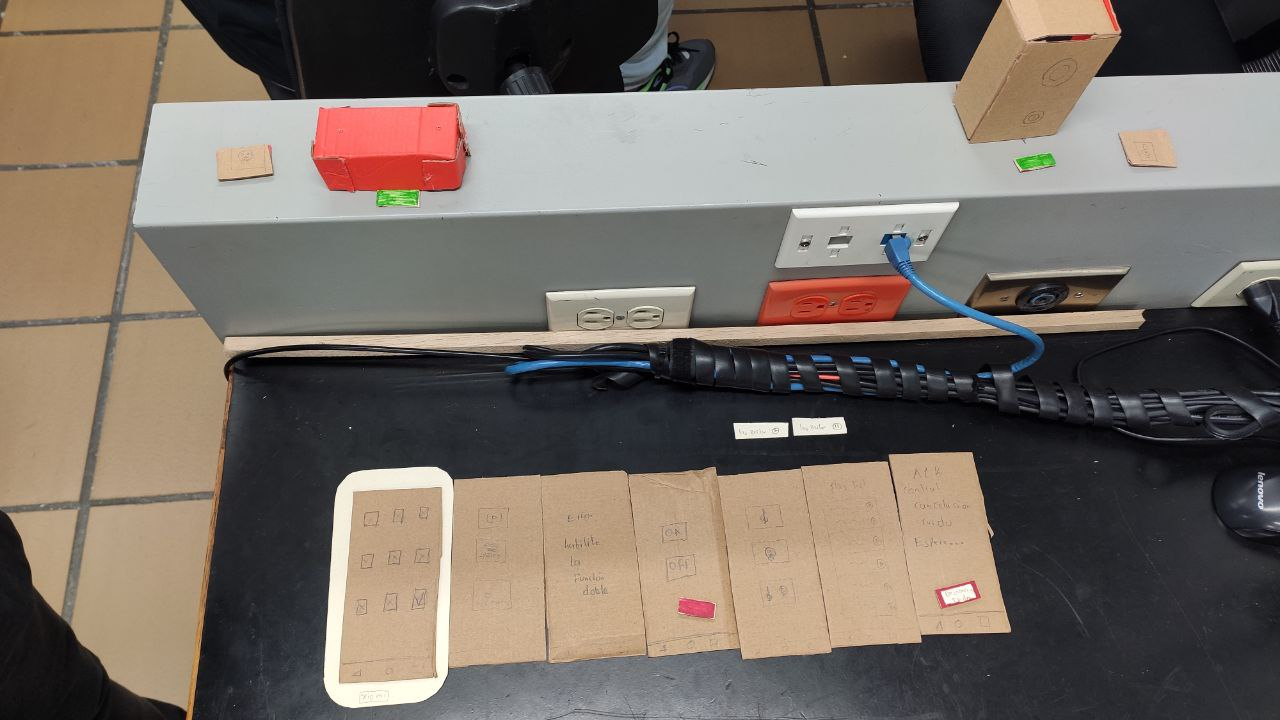
\includegraphics[width=16cm]{imagenes/photo1643818599.jpeg}
    \caption{Prototipo de la idea}
    \label{fig:galaxy}
\end{figure}

En esta imagen se ve una aplicación donde el usuario puede escoger 3 opciones, una opción que redirige al usuario  a distintas plataformas de musica, otra opción para activar la cancelación de ruido, esta opción activa los micrófonos instalados para cancelar el ruido y por ultimo la opción doble donde el bafle reproduce la musica pero también las ondas negadas del ruido para cancelar el ruido.\bigskip


Después de dejar que varias personas utilizaran el prototipo y nos dieran su retroalimentación  se ve que es un buen producto que muchas personas estarían dispuestos a comprar, una de las ideas que nos dieron que puede funcionar fue la de permitir que la cancelación de ruido funcione con cualquier artefacto de sonido, no solamente con los inteligentes y ya que el negocio no estaría en la venta del producto o los bafles sino en el mantenimiento de la aplicación y la personalizaron de los productos.\bigskip

\section{Revisión problema: }
Luego del diseño del prototipo, se procede a mirar de una forma más amplia las problemáticas que dicho dispositivo podría solucionar, revisando tanto la accesibilidad en el mercado, nicho de mercado y complejidad de construcción de cada solución.\bigskip

Para nuestro caso existen 3 problemáticas directas y una indirecta que es en caso tal que el dispositivo ya este en el mercado. Con ello utilizamos niveles de dolor de 1 al 5, dichos niveles significan que tan fácil, accesible o necesario es cada uno de los ítem presentados en la primera fila, siendo 5 un dolor máximo y 1 el mínimo.\bigskip

\begin{figure}[H]
    \centering
    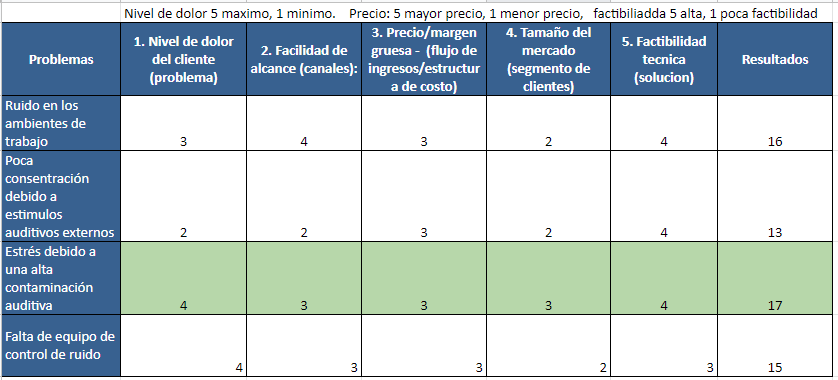
\includegraphics[scale = 0.7]{imagenes/cuadro.PNG}
    \caption{Revisión de problema}
    \label{fig:my_label}
\end{figure}

Luego de la revisión de problemas, podemos concluir que el mejor problema que podemos solucionar es el estrés debido a una alta contaminación auditiva, problema que se encuentra resaltado en la Figura 2.\bigskip


\section{Preparacion para PUV (Prepuesta única de valor):}

Para el desarrollo de la propuesta única de valor se desarrollaron distintas herramientas como lo es la herramienta DOFA o el diagrama mostrado en la siguiente imagen que nos permite entender como esta nuestro producto en comparación con el mercado.

\begin{figure}[H]
    \centering
    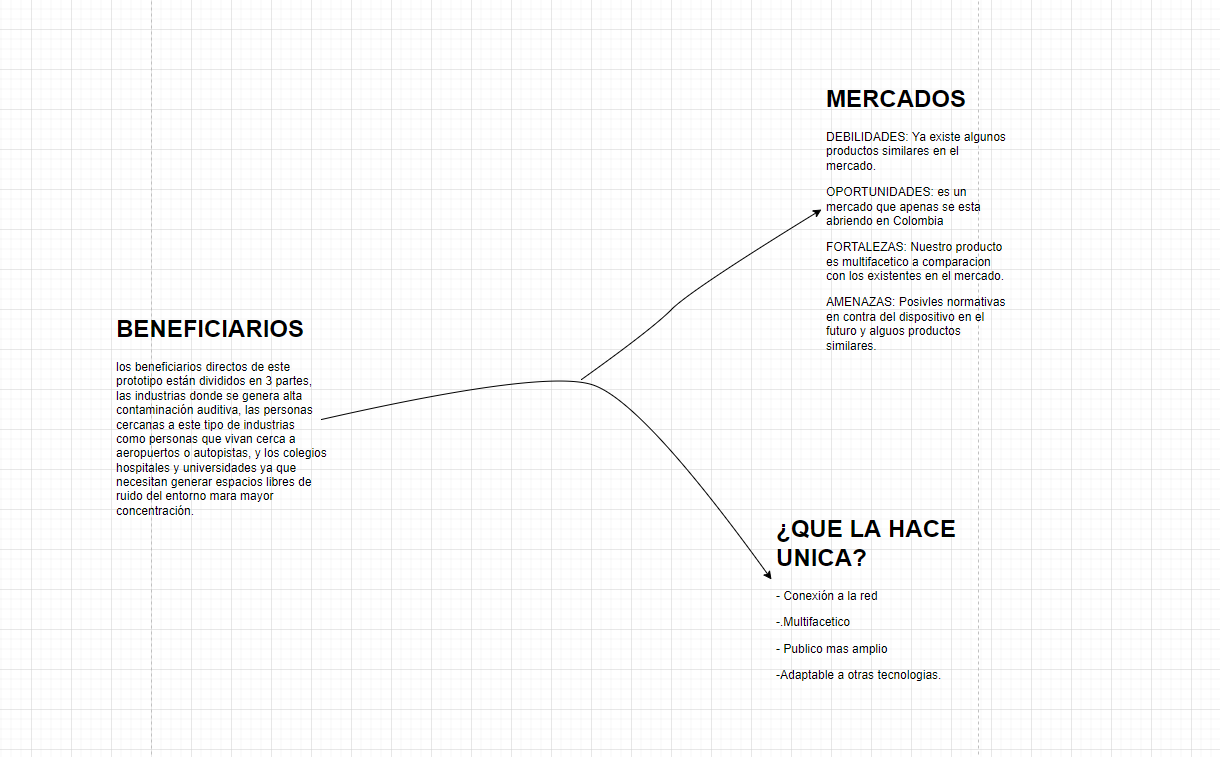
\includegraphics[scale = 0.5]{imagenes/PUV1.png}
    \caption{Espina de pescado}
    \label{fig:my_label}
\end{figure}


\section{PUV :}
Después de tener mayor claridad e información del problema y el mercado, podemos empezar a marcar algunos diferenciales de nuestro producto respecto a los productos que ya existen, dichos diferenciales son:
\begin{itemize}
    \item Un producto polifacético, ya que incorpora un sistema de cancelación de ruido y adicionalmente posee conexión a la red, lo que permite que el usuario pueda escuchar música de \textbf{mas de 3 plataformas}. 
    
    \item Para dar un valor en la parte estética se tienen \textbf{más de 10} carcasas para proteger el dispositivo.
    
    \item El producto sirve para \textbf{más de una persona}.\bigskip
\end{itemize}


\section{Lean canvas:}
Por medio de la herramienta para modelos de negocio LEAN CANVAS, se desarrolla un cuadro comparativo en donde se puede ver la robustez no solo del producto sino de todo un modelo de negocio al rededor de dicho producto, esto lo hacemos evaluando el producto, el cliente y el mercado con sus costos y ganancias  como se ve en el siguiente cuadro.

\begin{figure}[H]
    \centering
    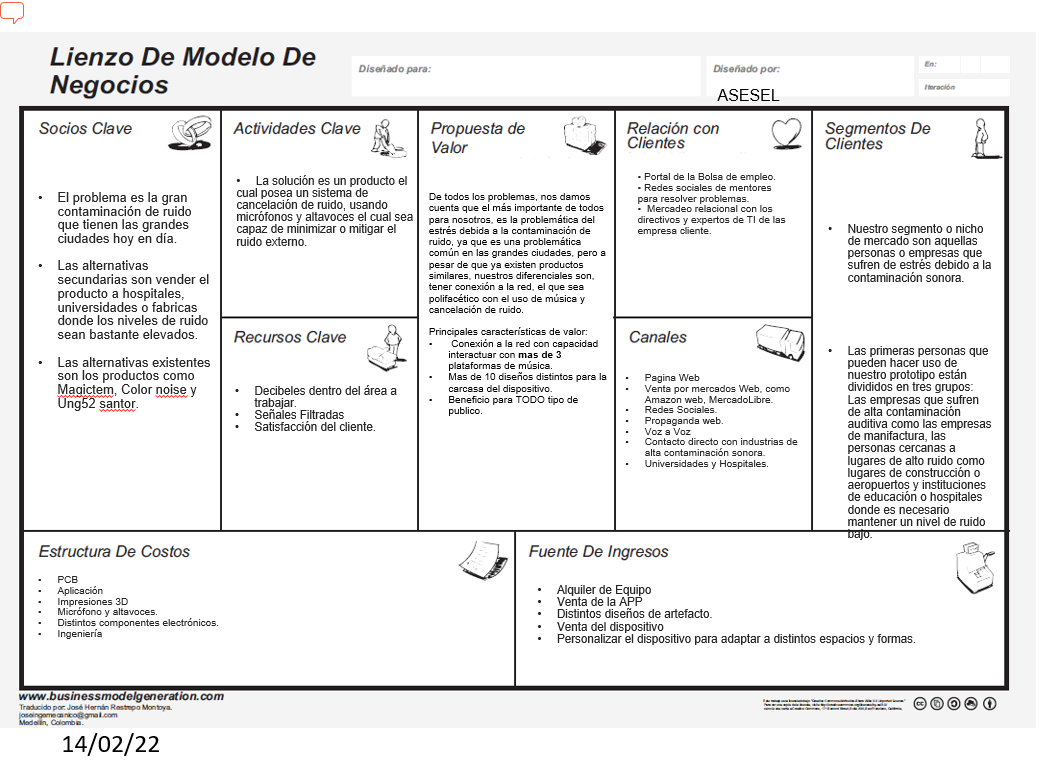
\includegraphics[scale = 0.5]{imagenes/LEAN-CANVAS.png}
    \caption{CANVAS AJUSTADO}
    \label{fig:my_label}
\end{figure}

\section{Costos}
Para el desarrollo de los costos se utilizo una Plantilla donde se organizaron los distintos costos, Donde se tuvo en cuenta que trabajaran dos ingenieros, el costo de los materiales del producto, es importante también aclarar que se utilizara software libre para bajar costos de producción y tampoco se utilizaran servicios especiales de ensamble, por ultimo también se tuvo en cuenta los costos fijos y dio como resultado un costo total contando IVA e impuestos.

\begin{figure}[H]
    \centering
    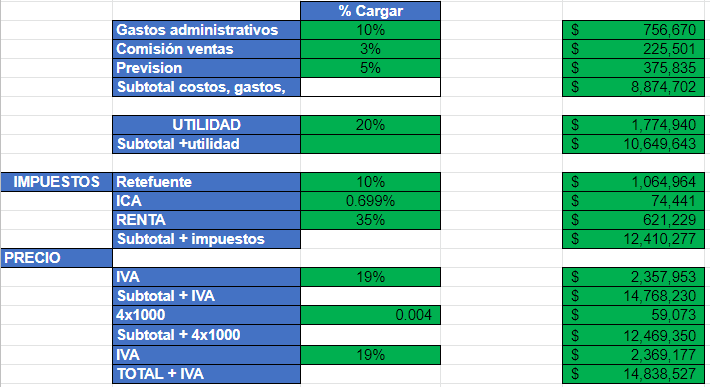
\includegraphics[scale = 0.9]{imagenes/costos.PNG}
    \caption{Cuadro de Costos}
    \label{fig:my_label}
\end{figure}


\section{Precio}
Para el desarrollo de esta parte se realizo tres estrategias para poder calcular el precio final al usuario, estas estrategias son \textbf{COST PLUS}.\bigskip , \textbf{MARKET MINUS}.\bigskip y \textbf{VALUE ADDED}.\bigskip en donde se miran distintas formas de generar un costo.

\begin{itemize}
    \item para desarrollar la estrategia \textbf{COST PLUS}.\bigskip se mira que el costo mensual para desarrollar un dispositivo es de alrededor de los 4 millones de pesos, analizando el mercado, la competencia y como nuestra incursión en este mercado podría impactar decidimos poner una utilidad del 20 por ciento sobre el costo del producto, lo cual da alrededor de 5 millones de pesos.
    
    \item Para el desarrollo de la metodología \textbf{MARKET MINUS}.\bigskip  primero se hace un estudio de mercado, como se explico anterior mete este producto esta relativamente nuevo en el mercado y la competencia pone precios grandes o no tiene todas las funcionalidades que nosotros tenemos, y viendo que el mercado colombiano es altamente competitivo y con el fin de posicionar nuestra marca en el mercado hemos decidido poner un precio un 5 por ciento menor que de la competencia quedando como total dando como total 320000.
    
    \item Para el desarrollo de la ultima metodología para desarrollar el precio llamada \textbf{VALUE ADDED}. Se mira las características y cualidades de los productos de la competencia, revisamos nuestra prepuesta de valor y esto como se diferencia de las otras compañías, basado en esto y viendo que nuestro producto tiene cualidades muy llamativas se agrega un 10 por ciento al precio del mercado dando como resultado 370000.
\end{itemize}


\begin{figure}[H]
    \centering
    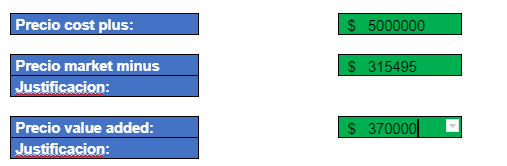
\includegraphics[scale = 0.9]{imagenes/precios.PNG}
    \caption{Cuadro de Precios}
    \label{fig:my_label}
\end{figure}





\label{sec:conclusions}



% Escriba su texto aquí

\nocite{*}
\bibliographystyle{IEEEtran}


\end{document}


